\documentclass[../sparc.tex]{subfiles}
\graphicspath{{\subfix{../images/}}}
\begin{document}

%%%%%%%%%%%%%%%%%%%%%%%%%%%%%%%%%%%%%%%%%%%%%%%%%%%%%%%%%%%%%%%%%%%%%%%%%%%%%%%%
\section{Длина волны}

При создании ``мигающего светодиода'' мы попеременно подавали на цифровой порт
сигналы \texttt{HIGH} и \texttt{LOW}, с указанием задержки (в миллисекундах).
Если мы посмотрим на вид сигнала на цифровом порту во времени (скажем, с помощью
осциллографа), то увидим график, примерно как на рис.
\ref{fig:blinking-led-graph}.

\begin{figure}[ht]
  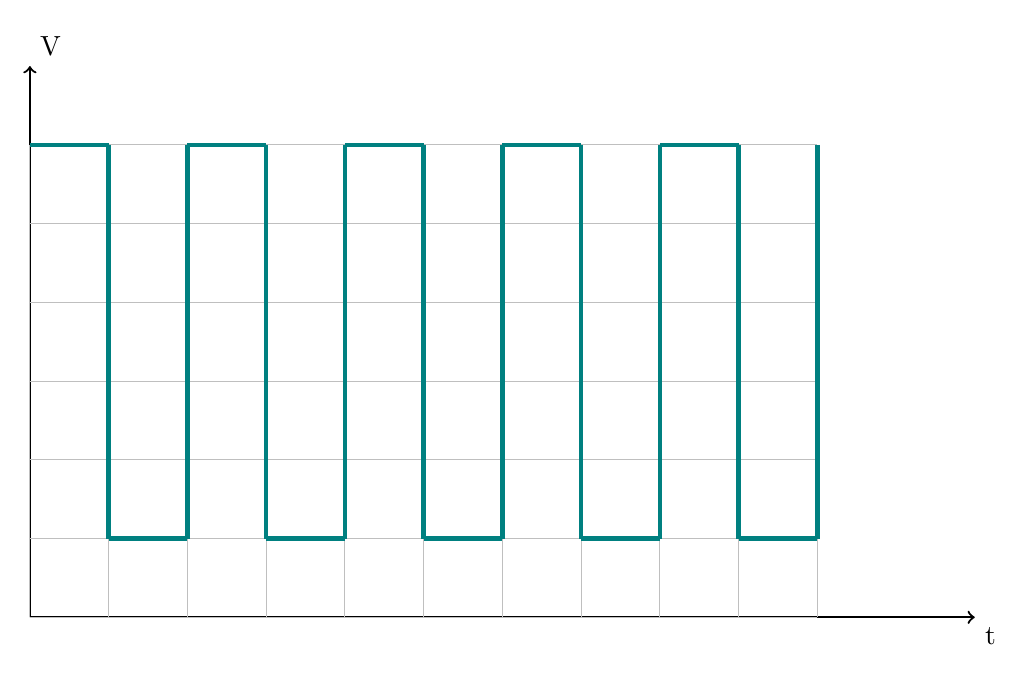
\begin{tikzpicture}
    \draw[thick, ->] (0, 0) -- (12, 0) node[anchor=north west] {t};
    \draw[thick, ->] (0, 0) -- (0,  7) node[anchor=south west] {V};
    \draw[lightgray] (0, 0) grid (10, 6);
    \foreach \x in {0, 2, ..., 8} {
      \draw[ultra thick, teal] (\x, 6) -- (\x + 1, 6);
      \draw[ultra thick, teal] (\x + 1, 6) -- (\x + 1, 1);
      \draw[ultra thick, teal] (\x + 1, 1) -- (\x + 2, 1);
      \draw[ultra thick, teal] (\x + 2, 1) -- (\x + 2, 6);
    }
  \end{tikzpicture}
  \caption{Графическое отображение сигнала, меняющегося во времени, на цифровом
    порту.}
  \label{fig:blinking-led-graph}
\end{figure}

Где \emph{длина периода} -- расстояние между двумя ближайшими друг к другу
точками в пространстве, в которых колебания происходят в одинаковой фазе.

Зная длину периода, можно рассчитать \emph{частоту колебаний}, и наоборот --
зная частоту, можно рассчитать длину волны.

При работе с ШИМ мы будем использовать длину периода, заданную в микросекундах
(мкс). 1 микросекунда -- это одна миллионная часть секунды. Для краткости записи
подобных маленьких величин часто используется возведение числа 10 в
отрицательную степень. Ниже приведена таблица с указанием различных долей
секунды\footnote{Для полного списка кратных и дольных единиц см. статью
\href{https://ru.wikipedia.org/wiki/\%D0\%A1\%D0\%B5\%D0\%BA\%D1\%83\%D0\%BD\%D0\%B4\%D0\%B0}{Секунда}
в Википедии.}:

\begin{tabular}{p{4cm}|p{4cm}|p{6cm}}
  Название & Величина & Пример \\
  \hline \hline
  секунда (с) & $ 1 с $ или $ 10^0 с $ & $ 500 * 10^{0} = 500 с $ \\
  \hline
  миллисекунда (мс) & $ 0.001 c $ или $ 10^{-3} c $ & $ 500 * 10^{-3} = 500 мс $ \\
  \hline
  микросекунда (мкс) & $ 0.000001 c $ или $ 10^{-6} c $ & $ 500 * 10^{-6} = 500 мкс $ \\
  \hline
  наносекунда (нс) & $ 0.000000001 c $ или $ 10^{-9} с $ & $ 500 * 10^{-9} = 500 нс $
\end{tabular}

\end{document}
